\iffalse
This file is protected by Copyright. Please refer to the COPYRIGHT file
distributed with this source distribution.

This file is part of OpenCPI <http://www.opencpi.org>

OpenCPI is free software: you can redistribute it and/or modify it under the
terms of the GNU Lesser General Public License as published by the Free Software
Foundation, either version 3 of the License, or (at your option) any later
version.

OpenCPI is distributed in the hope that it will be useful, but WITHOUT ANY
WARRANTY; without even the implied warranty of MERCHANTABILITY or FITNESS FOR A
PARTICULAR PURPOSE. See the GNU Lesser General Public License for more details.

You should have received a copy of the GNU Lesser General Public License along
with this program. If not, see <http://www.gnu.org/licenses/>.
\fi

%----------------------------------------------------------------------------------------
% Required document specific properties
%----------------------------------------------------------------------------------------
\def\comp{zero\_{}padding}
\edef\ecomp{zero_padding}
\def\Comp{Zero Padding}
\def\docTitle{\Comp{} Component Data Sheet}
\def\snippetpath{../../../../../../doc/av/tex/snippets}
%----------------------------------------------------------------------------------------
% Global latex header (this must be after document specific properties)
%----------------------------------------------------------------------------------------
\iffalse
This file is protected by Copyright. Please refer to the COPYRIGHT file
distributed with this source distribution.

This file is part of OpenCPI <http://www.opencpi.org>

OpenCPI is free software: you can redistribute it and/or modify it under the
terms of the GNU Lesser General Public License as published by the Free Software
Foundation, either version 3 of the License, or (at your option) any later
version.

OpenCPI is distributed in the hope that it will be useful, but WITHOUT ANY
WARRANTY; without even the implied warranty of MERCHANTABILITY or FITNESS FOR A
PARTICULAR PURPOSE. See the GNU Lesser General Public License for more details.

You should have received a copy of the GNU Lesser General Public License along
with this program. If not, see <http://www.gnu.org/licenses/>.
\fi

% Sets OpenCPI Version used throughout all the docs. This is updated by
% scripts/update-release.sh when a release is being made and must not
% be changed manually.
\def\ocpiversion{v2.2.0}

\documentclass{article}
\author{}  % Force author to be blank
\date{OpenCPI Release:\ \ \ocpiversion}  % Force date to be blank and override date with version
\title{OpenCPI\\\docTitle}  % docTitle must be defined before including this file
%----------------------------------------------------------------------------------------
% Paper size, orientation and margins
%----------------------------------------------------------------------------------------
\usepackage{geometry}
\geometry{
  letterpaper,  % paper type
  portrait,     % text direction
  left=.75in,   % left margin
  top=.75in,    % top margin
  right=.75in,  % right margin
  bottom=.75in  % bottom margin
}
%----------------------------------------------------------------------------------------
% Header/Footer
%----------------------------------------------------------------------------------------
\usepackage{fancyhdr} \pagestyle{fancy}  % required for fancy headers
\renewcommand{\headrulewidth}{0.5pt}
\renewcommand{\footrulewidth}{0.5pt}
\lhead{\small{\docTitle}}
\rhead{\small{OpenCPI}}
%----------------------------------------------------------------------------------------
% Various packages
%----------------------------------------------------------------------------------------
\usepackage{amsmath}
\usepackage[page,toc]{appendix}  % for appendix stuff
\usepackage{enumitem}
\usepackage{graphicx}   % for including pictures by file
\usepackage{hyperref}   % for linking urls and lists
\usepackage{listings}   % for coding language styles
\usepackage{pdflscape}  % for landscape view
\usepackage{pifont}     % for sideways table
\usepackage{ragged2e}   % for justify
\usepackage{rotating}   % for sideways table
\usepackage{scrextend}
\usepackage{setspace}
\usepackage{subfig}
\usepackage{textcomp}
\usepackage[dvipsnames,usenames]{xcolor}  % for color names see https://en.wikibooks.org/wiki/LaTeX/Colors
\usepackage{xstring}
\uchyph=0  % Never hyphenate acronyms like RCC
\renewcommand\_{\textunderscore\allowbreak}  % Allow words to break/newline on underscores
%----------------------------------------------------------------------------------------
% Table packages
%----------------------------------------------------------------------------------------
\usepackage[tableposition=top]{caption}
\usepackage{float}
\floatstyle{plaintop}
\usepackage{longtable}  % for long possibly multi-page tables
\usepackage{multicol}   % for more advanced table layout
\usepackage{multirow}   % for more advanced table layout
\usepackage{tabularx}   % c=center,l=left,r=right,X=fill
% These define tabularx columns "C" and "R" to match "X" but center/right aligned
\newcolumntype{C}{>{\centering\arraybackslash}X}
\newcolumntype{M}[1]{>{\centering\arraybackslash}m{#1}}
\newcolumntype{P}[1]{>{\centering\arraybackslash}p{#1}}
\newcolumntype{R}{>{\raggedleft\arraybackslash}X}
%----------------------------------------------------------------------------------------
% Block Diagram / FSM Drawings
%----------------------------------------------------------------------------------------
\usepackage{tikz}
\usetikzlibrary{arrows,decorations.markings,fit,positioning,shapes}
\usetikzlibrary{automata}  % used for the fsm
\usetikzlibrary{calc}      % for duplicating clients
\usepgfmodule{oo}          % to define a client box
%----------------------------------------------------------------------------------------
% Colors Used
%----------------------------------------------------------------------------------------
\usepackage{colortbl}
\definecolor{blue}{rgb}{.7,.8,.9}
\definecolor{ceruleanblue}{rgb}{0.16, 0.32, 0.75}
\definecolor{cyan}{rgb}{0.0,0.6,0.6}
\definecolor{darkgreen}{rgb}{0,0.6,0}
\definecolor{deepmagenta}{rgb}{0.8, 0.0, 0.8}
\definecolor{maroon}{rgb}{0.5,0,0}
%----------------------------------------------------------------------------------------
% Define where to hyphenate
%----------------------------------------------------------------------------------------
\hyphenation{Cent-OS}
\hyphenation{install-ation}
%----------------------------------------------------------------------------------------
% Define Commands & Rename Commands
%----------------------------------------------------------------------------------------
\newcommand{\code}[1]{\texttt{#1}}  % For inline code snippet or command line
\newcommand{\sref}[1]{Section~\ref{#1}}  % To quickly reference a section
\newcommand{\todo}[1]{\textcolor{red}{TODO: #1}\PackageWarning{TODO:}{#1}}  % To do notes
\renewcommand{\contentsname}{Table of Contents}
\renewcommand{\listfigurename}{List of Figures}
\renewcommand{\listtablename}{List of Tables}

% This gives a link to gitlab.io document. By default, it outputs the filename.
% You can optionally change the link, e.g.
% \githubio{FPGA\_Vendor\_Tools\_Installation\_Guide.pdf} vs.
% \githubio[\textit{FPGA Vendor Tools Installation Guide}]{FPGA\_Vendor\_Tools\_Installation\_Guide.pdf}
% or if you want the raw ugly URL to come out, \githubioURL{FPGA_Vendor_Tools_Installation_Guide.pdf}
\newcommand{\githubio}[2][]{% The default is for FIRST param!
\href{http://opencpi.gitlab.io/releases/\ocpiversion/docs/#2}{\ifthenelse{\equal{#1}{}}{\texttt{#2}}{#1}}}
\newcommand{\gitlabcom}[2][]{% The default is for FIRST param!
\href{http://gitlab.com/opencpi/#2}{\ifthenelse{\equal{#1}{}}{\texttt{#2}}{#1}}}
\newcommand{\githubioURL}[1]{\url{http://opencpi.gitlab.io/releases/\ocpiversion/docs/#1}}
% Lastly, if you want a SINGLE leading path stripped, e.g. assets/X.pdf => X.pdf:
\newcommand{\githubioFlat}[1]{%
\StrBehind{#1}{/}[\den]%
\href{http://opencpi.gitlab.io/releases/\ocpiversion/docs/#1}{\texttt{\den}}%
}
%----------------------------------------------------------------------------------------
% VHDL Coding Language Style
% modified from: http://latex-community.org/forum/viewtopic.php?f=44&t=22076
%----------------------------------------------------------------------------------------
\lstdefinelanguage{VHDL}
{
  basicstyle=\ttfamily\footnotesize,
  columns=fullflexible,keepspaces,  % https://tex.stackexchange.com/a/46695/87531
  keywordstyle=\color{ceruleanblue},
  commentstyle=\color{darkgreen},
  morekeywords={
    library, use, all, entity, is, port, in, out, end, architecture, of,
    begin, and, signal, when, if, else, process, end,
  },
  morecomment=[l]--
}
%----------------------------------------------------------------------------------------
% XML Coding Language Style
% modified from http://tex.stackexchange.com/questions/10255/xml-syntax-highlighting
%----------------------------------------------------------------------------------------
\lstdefinelanguage{XML}
{
  basicstyle=\ttfamily\footnotesize,
  columns=fullflexible,keepspaces,
  morestring=[s]{"}{"},
  morecomment=[s]{!--}{--},
  commentstyle=\color{darkgreen},
  moredelim=[s][\color{black}]{>}{<},
  moredelim=[s][\color{cyan}]{\ }{=},
  stringstyle=\color{maroon},
  identifierstyle=\color{ceruleanblue}
}
%----------------------------------------------------------------------------------------
% DIFF Coding Language Style
% modified from http://tex.stackexchange.com/questions/50176/highlighting-a-diff-file
%----------------------------------------------------------------------------------------
\lstdefinelanguage{diff}
{
  basicstyle=\ttfamily\footnotesize,
  columns=fullflexible,keepspaces,
  breaklines=true,                            % wrap text
  morecomment=[f][\color{ceruleanblue}]{@@},  % group identifier
  morecomment=[f][\color{red}]-,              % deleted lines
  morecomment=[f][\color{darkgreen}]+,        % added lines
  morecomment=[f][\color{deepmagenta}]{---},  % Diff header lines (must appear after +,-)
  morecomment=[f][\color{deepmagenta}]{+++},
}
%----------------------------------------------------------------------------------------
% Python Coding Language Style
%----------------------------------------------------------------------------------------
\lstdefinelanguage{python}
{
  basicstyle=\ttfamily\footnotesize,
  columns=fullflexible,keepspaces,
  keywordstyle=\color{ceruleanblue},
  commentstyle=\color{darkgreen},
  stringstyle=\color{orange},
  morekeywords={
    print, if, sys, len, from, import, as, open,close, def, main, for, else,
    write, read, range,
  },
  comment=[l]{\#}
}
%----------------------------------------------------------------------------------------
% Fontsize Notes in order from smallest to largest
%----------------------------------------------------------------------------------------
%    \tiny
%    \scriptsize
%    \footnotesize
%    \small
%    \normalsize
%    \large
%    \Large
%    \LARGE
%    \huge
%    \Huge

\graphicspath{{figures/}}
%----------------------------------------------------------------------------------------

\begin{document}
\maketitle
\thispagestyle{empty}
\newpage

\def\name{\comp}
\def\workertype{Application}
\def\version{\ocpiversion}
\def\releasedate{4/2019}
\def\componentlibrary{ocpi.assets.util\_{}comps}
\def\workers{\comp{}.hdl, \comp{}.rcc}
\def\testedplatforms{alst4, CentOS7, isim, Matchstiq-Z1(PL), ml605, modelsim, xilinx13\_{}3, xsim, ZedBoard(PL)}
\textbf{This worker will be deprecated in OpenCPI 2.0. Use the Zero Pad component for new designs.}\\
\section*{Summary - \Comp}
\begin{tabular}{|c|M{13.5cm}|}
  \hline
  \rowcolor{blue}
   & \\
  \hline
  Name              & \comp             \\
  \hline
  Worker Type       & \workertype       \\
  \hline
  OpenCPI Release   & \ocpiversion      \\
  \hline
  Last Update       & \releasedate      \\
  \hline
  Component Library & \componentlibrary \\
  \hline
  Workers           & \workers          \\
  \hline
  Tested Platforms  & \testedplatforms  \\
  \hline
\end{tabular}


\section*{Functionality}
\begin{flushleft}
	The {\Comp} component functions to expand input bits into signed Qm.n output samples within the range of $\pm1.0$, while inserting a variable number of zeros between output samples.\medskip

	Output data widths of 8/16/32/64 are supported resulting in (respectively) Q0.7, Q0.15, Q0.31, and Q0.63 output formats.
\end{flushleft}

\section*{Worker Implementation Details}
\begin{flushleft}
	The {\Comp} component couples the underlying data, or protocol, with the size of the output data plane in order to fully load a Qm.n sample within the output bus width. In order to be maximally flexible, the component does not define input/output protocols explicitly. Since the input is simply bits, the input protocol is irrelevant and defined by the component feeding the Zero Padding, such as the File Reader. The input/output data widths are defined at build time, which in turn define the respective input/output sample sizes.
\end{flushleft}

\section*{Theory}
\begin{flushleft}
	The Qm.n format defines the range to be $-2^{m}$ to $2^{m}-2^{-n}$, with a resolution of $2^{-n}$. For the Zero Padding component, m is equal to zero, while n is defined at compile-time and is equal to the size of the output data width minus one. For example, an output data width of 16 results in Q0.15 format, where numbers are in the range of $-1$ to $+0.999969482421875$ (almost $+1$) with a bit resolution of $0.000030517578125$.
\end{flushleft}

\section*{Block Diagrams}
\subsection*{Top level}
\begin{center}
	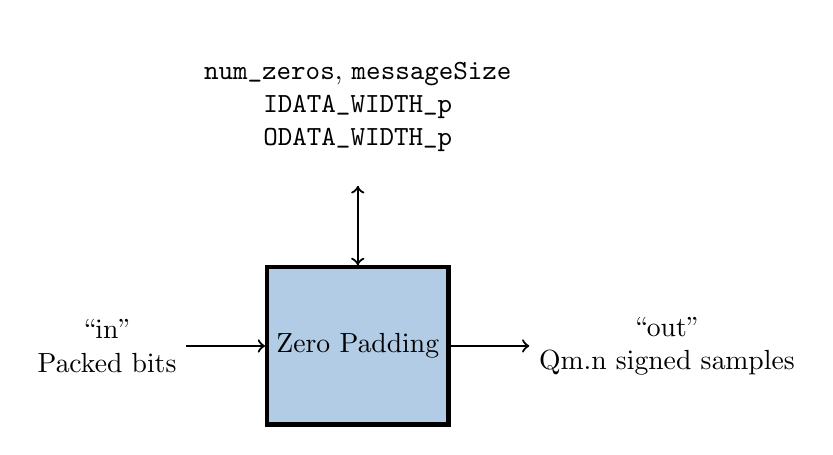
\begin{tikzpicture}[% List of styles applied to all, to override specify on a case-by-case
			every node/.style={
				align=center,  		% use this so that the "\\" for line break works
				minimum size=2cm	% creates space above and below text in rectangle
			},
			every edge/.style={draw,thick}
		]
		\node[rectangle,ultra thick,draw=black,fill=blue](R2){\Comp};
		\node[rectangle,draw=white,fill=white](R3)[left= of R2]{``in'' \\ Packed bits};
		\node[rectangle,draw=white,fill=white](R4)[right= of R2]{``out'' \\ Qm.n signed samples};
		\node[rectangle,draw=white,fill=white](R5)[above= of R2]{\verb+num_zeros+, \verb+messageSize+\\ \verb+IDATA_WIDTH_p+\\ \verb+ODATA_WIDTH_p+};
		\path[->]
		(R3)edge []	node [] {} (R2)
		(R2)edge []	node [] {} (R4)
		(R2)edge []	node [] {} (R5)
		(R5)edge []	node [] {} (R2)
		;
	\end{tikzpicture}
\end{center}\pagebreak

\subsection*{State Machine}
\begin{flushleft}
	Two finite-state machines (FSMs) are implemented by this worker. One FSM implements worker functionality while the other supports Zero-Length Messages.
\end{flushleft}
{\centering\captionsetup{type=figure}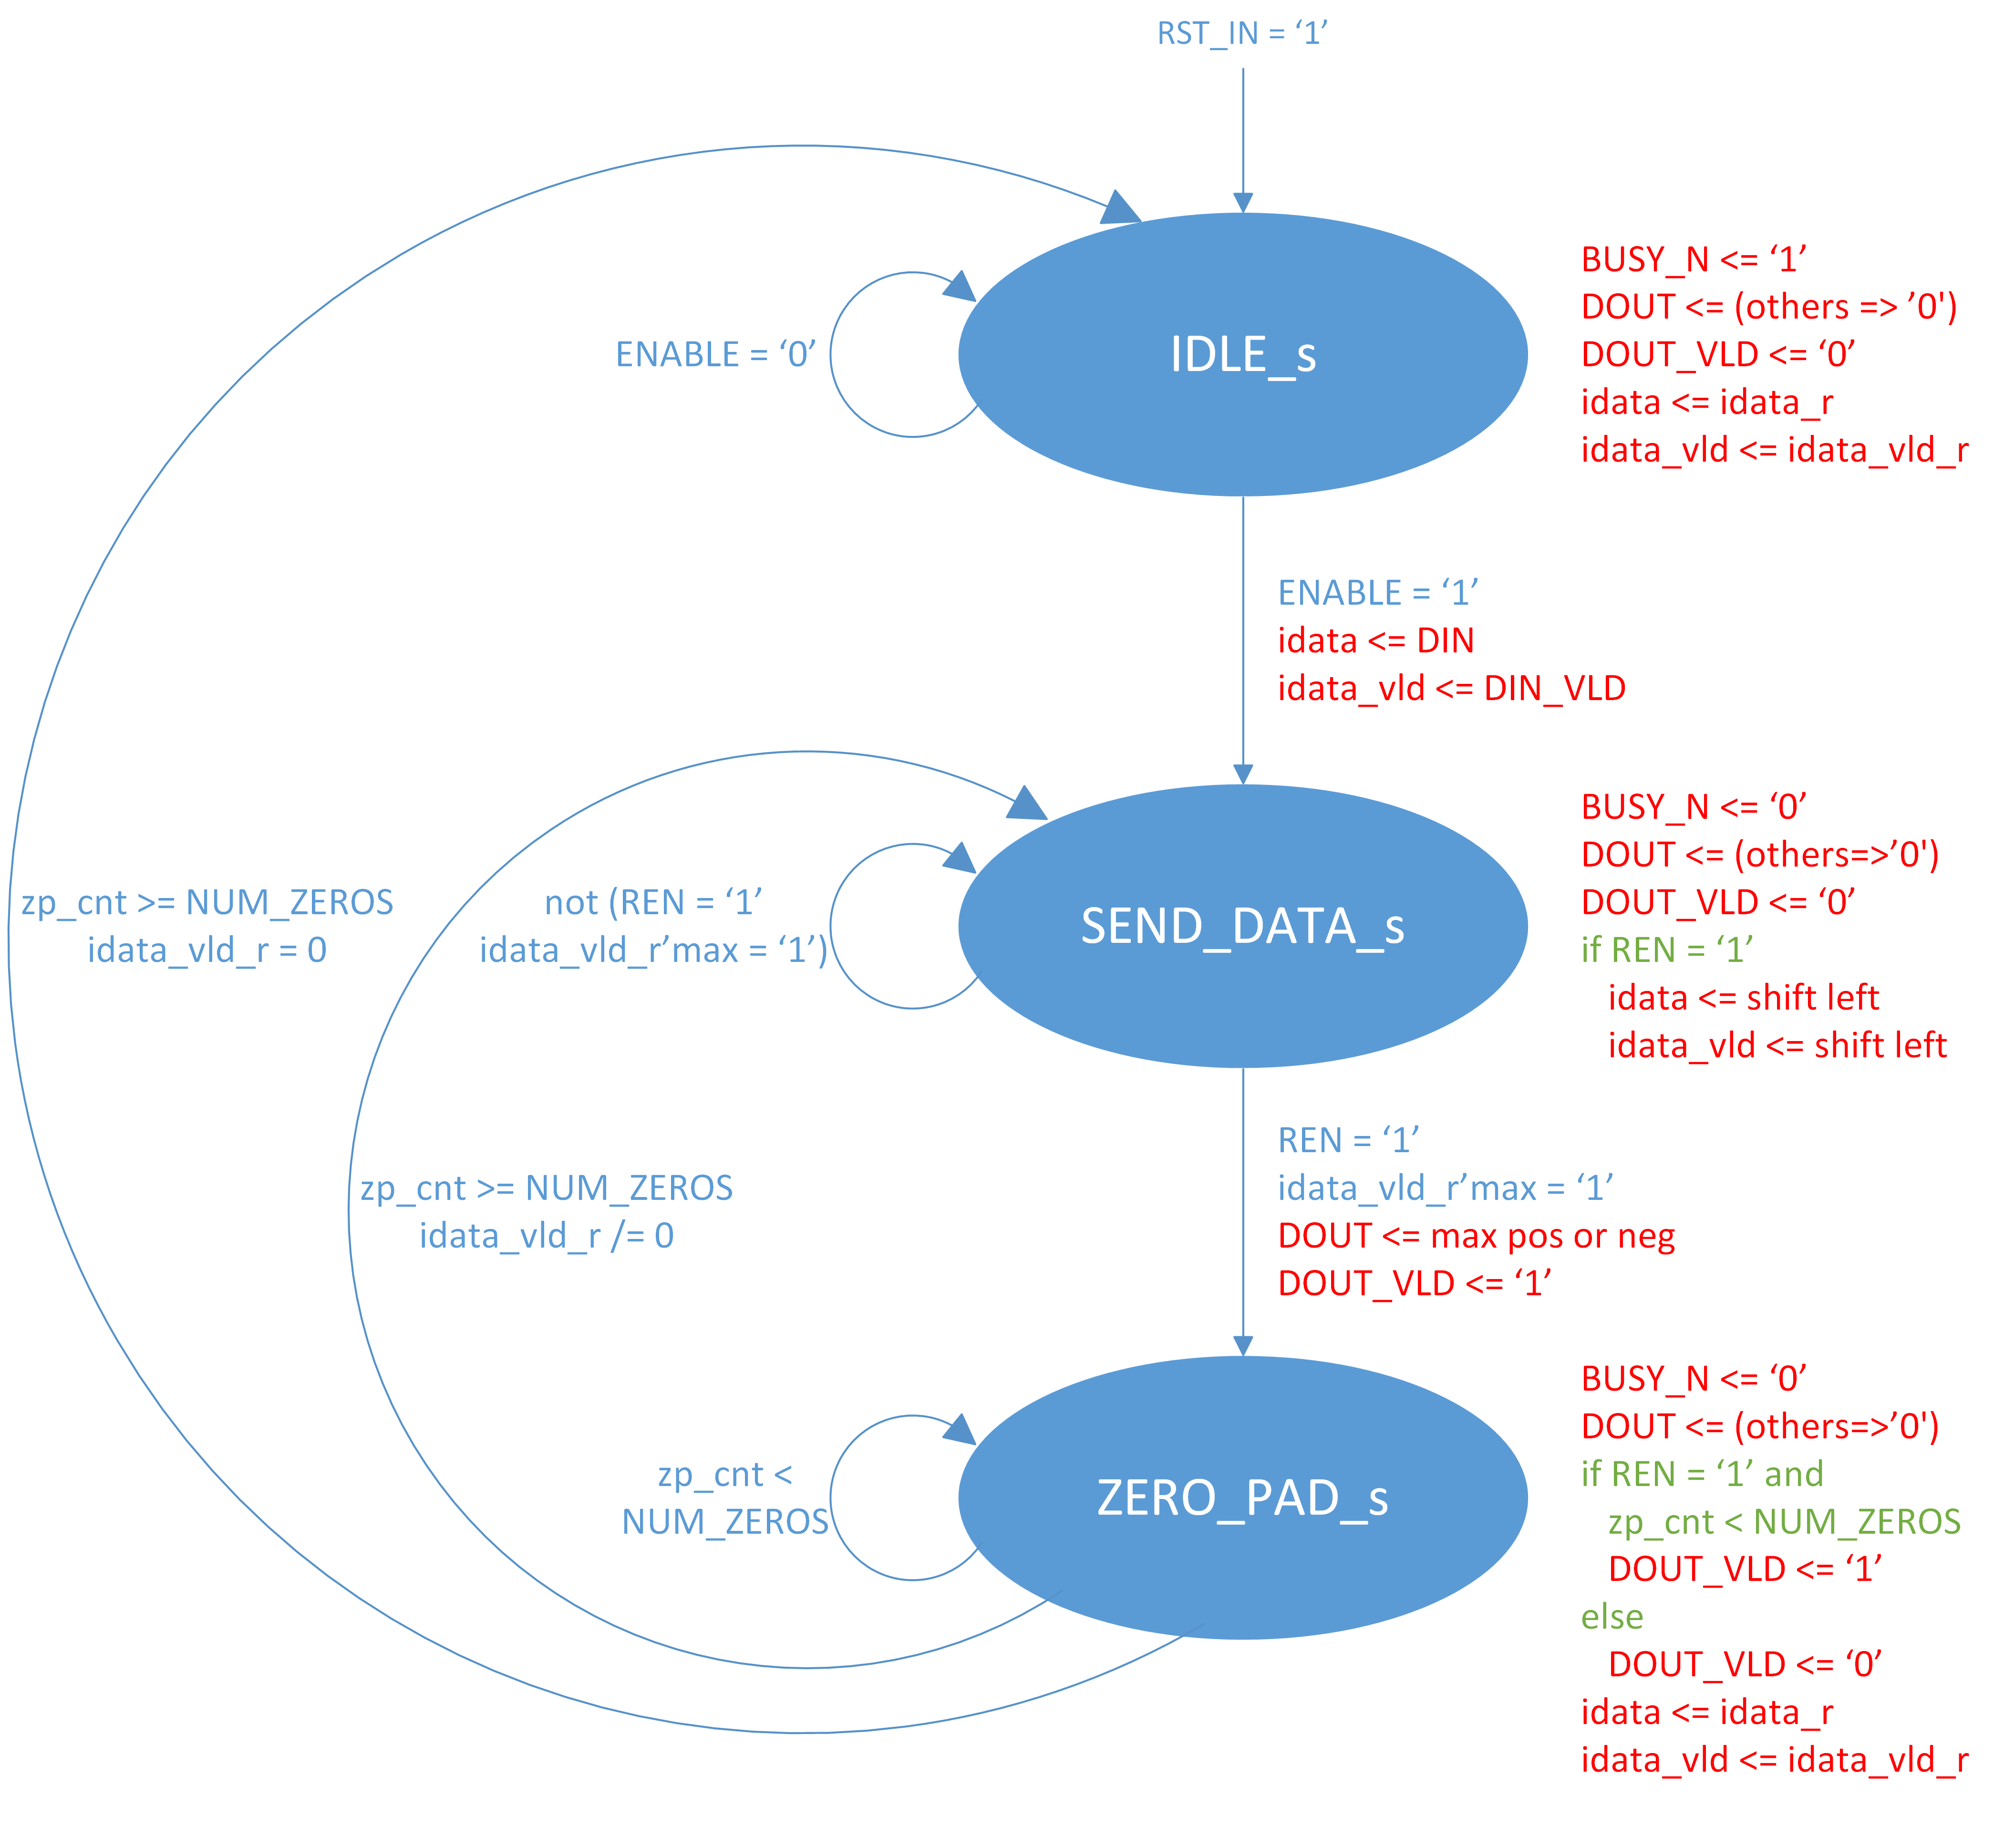
\includegraphics[scale=0.6]{zero_padding_fsm}\par\captionof{figure}{Zero Padding FSM}\label{fig:zp_fsm}} \hfill \break
{\centering\captionsetup{type=figure}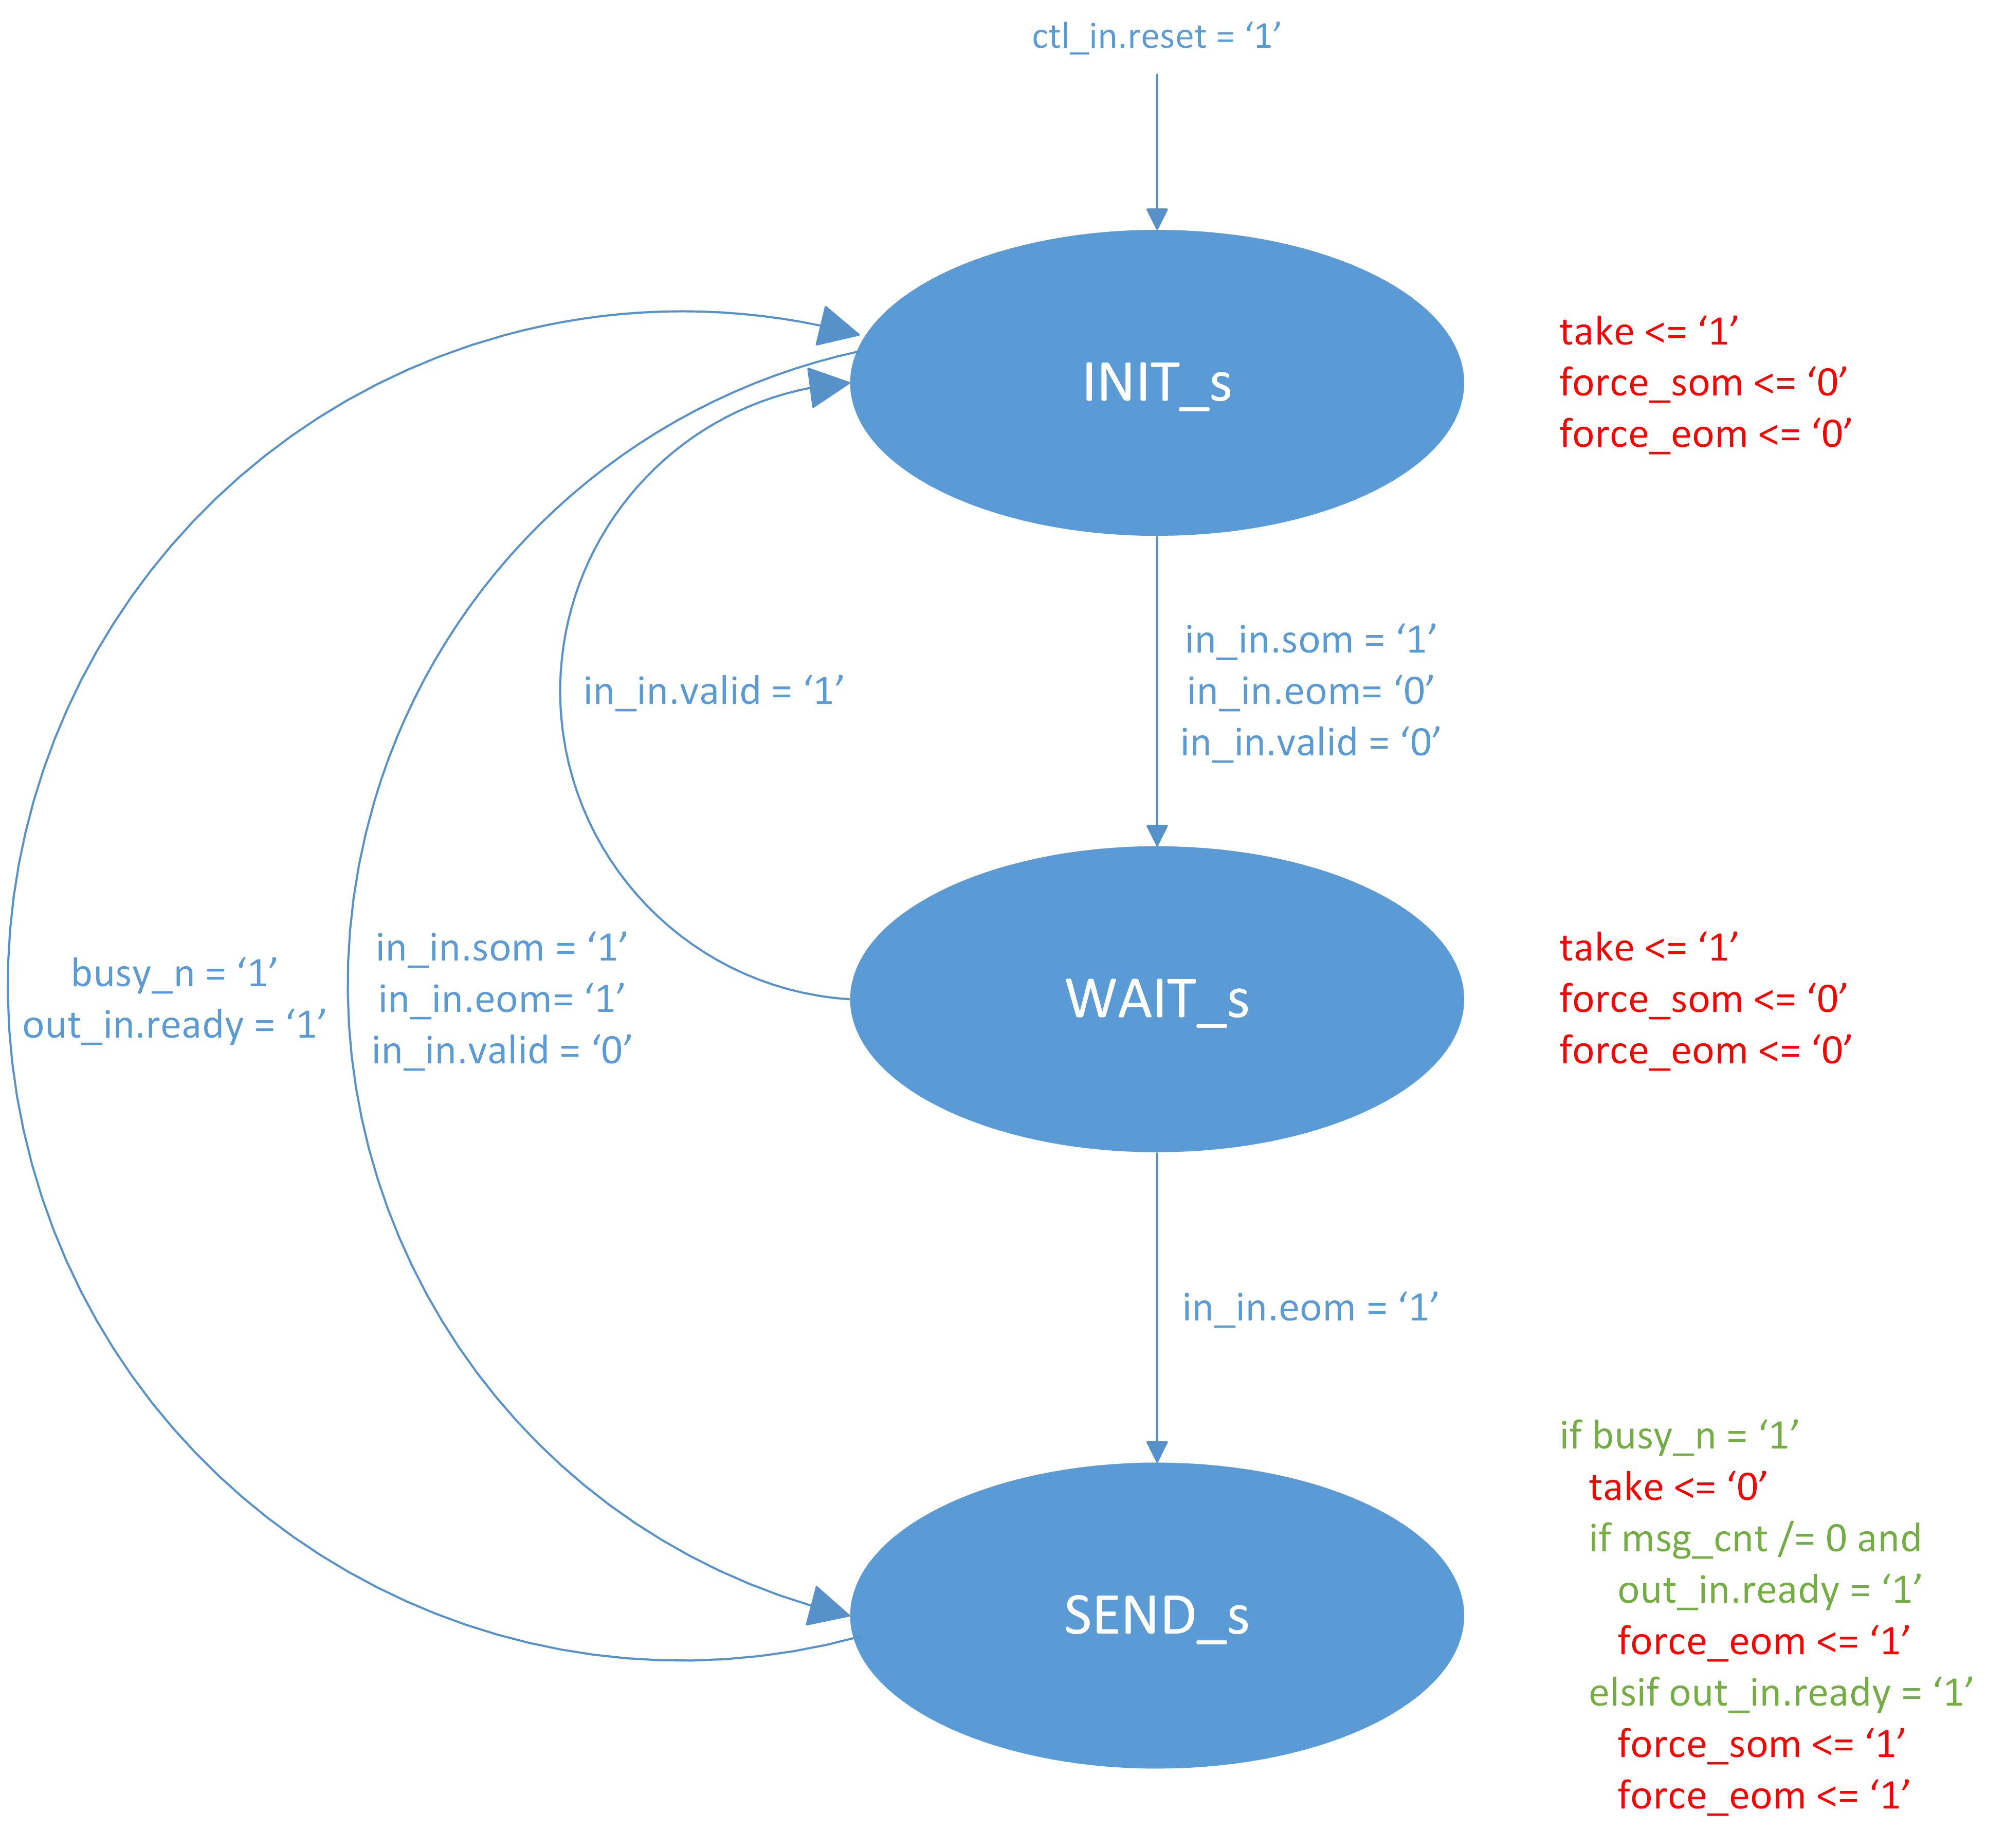
\includegraphics[scale=0.7]{zlm_fsm}\par\captionof{figure}{Zero-Length Message FSM}\label{fig:zlm_fsm}}

\section*{Source Dependencies}
\subsection*{\comp.rcc}
\begin{itemize}
	\item projects/assets/components/util\_comps/zero\_padding.rcc/zero\_padding.cc
\end{itemize}
\subsection*{\comp.hdl}
\begin{itemize}
	\item projects/assets/components/util\_comps/zero\_padding.hdl/zero\_padding.vhd
	\item projects/assets/hdl/primitives/util\_prims/util\_prims\_pkg.vhd
	      \subitem projects/assets/hdl/primitives/util\_prims/zp/src/zero\_padding\_gen.vhd
\end{itemize}

\begin{landscape}
	\section*{Component Spec Properties}
	\begin{scriptsize}
		\begin{tabular}{|p{2cm}|p{1.5cm}|c|c|c|p{1.5cm}|p{1cm}|p{7cm}|}
			\hline
			\rowcolor{blue}
			Name                 & Type   & SequenceLength & ArrayDimensions & Accessibility       & Valid Range & Default & Usage                                                 \\
			\hline
			\verb+IDATA_WIDTH_p+ & ulong  & -              & -               & Readable, Parameter & 8/16/32/64  & 32      & Input port data width                                 \\
			\hline
			\verb+ODATA_WIDTH_p+ & ulong  & -              & -               & Readable, Parameter & 8/16/32/64  & 32      & Output port data width                                \\
			\hline
			\verb+num_zeros+     & ushort & -              & -               & Readable, Writable  & Standard    & -       & number of zeros to be inserted between output samples \\
			\hline
			\verb+messageSize+   & ushort & -              & -               & Readable, Writable  & Standard    & 8192    & number of bytes in output message \\
			\hline
		\end{tabular}
	\end{scriptsize}

	\section*{Worker Properties}
	\subsection*{\comp.hdl}
	\begin{scriptsize}
		\begin{tabular}{|p{2cm}|p{2cm}|p{1cm}|c|c|c|p{2cm}|p{1cm}|p{4cm}|}
			\hline
			\rowcolor{blue}
			Type     & Name                   & Type  & SequenceLength & ArrayDimensions & Accessibility       & Valid Range & Default & Usage                   \\
			\hline
			Property & \verb+MAX_NUM_ZEROS_p+ & ulong & -              & -               & Readable, Parameter & 0-255       & 255     & Maximum number of zeros \\
			\hline
		\end{tabular}
	\end{scriptsize}

	\section*{Component Ports}
	\begin{scriptsize}
		\begin{tabular}{|M{2cm}|M{1.5cm}|M{4cm}|c|c|M{9cm}|}
			\hline
			\rowcolor{blue}
			Name & Producer & Protocol & Optional & Advanced & Usage                                  \\
			\hline
			in   & False    & -        & False    & -        & Packed bits                            \\
			\hline
			out  & True     & -        & False    & -        & Qm.n signed samples representing ±1.0 \\
			\hline
		\end{tabular}
	\end{scriptsize}

	\section*{Worker Interfaces}
	\subsection*{\comp.hdl}
	\begin{scriptsize}
		\begin{tabular}{|M{2cm}|M{1.5cm}|M{4cm}|c|M{12cm}|}
			\hline
			\rowcolor{blue}
			Type            & Name & DataWidth            & Advanced & Usage                                       \\
			\hline
			StreamInterface & in   & \verb+IDATA_WIDTH_p+ & -        & Size defined by \verb+IDATA_WIDTH_p+        \\
			\hline
			StreamInterface & out  & \verb+ODATA_WIDTH_p+ & -        & Sample size defined by \verb+ODATA_WIDTH_p+ \\
			\hline
		\end{tabular}
	\end{scriptsize}
\end{landscape}

\section*{Control Timing and Signals}
\subsection*{\comp.hdl}
\begin{flushleft}
	This worker implementation uses the clock from the Control Plane and standard Control Plane signals.
\end{flushleft}

\begin{landscape}
\section*{Performance and Resource Utilization}
\subsubsection*{\comp.rcc}
Table entries are a result of compiling the worker with the following parameter/property set:\
\begin{itemize}
	\item \verb+IDATA_WIDTH_p+=16
	\item \verb+ODATA_WIDTH_p+=16
	\item \verb+num_zeros+=1
\end{itemize}
\begin{scriptsize}
	\begin{tabular}{|c|c|c|}
		\hline
		\rowcolor{blue}
		Processor Type                                & Processor Frequency & Run Function Time \\
		\hline
		linux-c6-x86\_64 Intel(R) Xeon(R) CPU E5-1607 & 3.00 GHz            & $\sim5$ ms        \\
		\hline
		linux-c7-x86\_64 Intel(R) Core(TM) i7-3630QM  & 2.40 GHz            & $\sim5$ ms        \\
		\hline
		linux-x13\_3-arm ARMv7 Processor rev 0 (v7l)    & 666 MHz             & $\sim21$ ms       \\
		\hline
	\end{tabular}
\section*{Worker Configuration Parameters}
\subsubsection*{\comp.hdl}
%\input{../../\ecomp.hdl/configurations.inc}
\end{scriptsize}
\subsubsection*{\comp.hdl}
%\input{../../\ecomp.hdl/utilization.inc}
\end{landscape}
\section*{Test and Verification}
\begin{flushleft}
	Both input and output data widths of 8/16/32/64 are supported and fully tested on both RCC and HDL worker implementations. The sixteen cross products of these input/output data width combinations are built for both RCC and HDL workers. These input/output combinations are each tested with \verb+num_zeros+ equal to 0, 1, 128, and 255 resulting in 64 test cases for both RCC and HDL workers.\medskip

	Input data is generated by a python script with an input parameter that defines the number of 32-bit words to produce. The input file consists of a repeating pattern of 0x0123456789ABCDEF. The number of 32-bit words for each test case is 2048, which results in 1024 64-bit samples, 2048 32-bit samples, 4096 16-bit samples, or 8192 8-bit samples. Thus for each test case the 64-bit test pattern is repeated 1024 times to produce a file of 65,536 bits (or 8192 bytes).\medskip

	The Zero Padding component inputs each bit and expands the bit into Qm.n format within the range of $\pm1.0$, where $m=0$, and n is defined by the width of the output data bus. Then \verb+num_zeros+ zeros are inserted between each output sample of width \verb+ODATA_WIDTH_p+.\medskip

	For verification, the output file is first checked that the data is not all zero, and is then checked for the expected length. Once these quick checks are made the output data is compared against expected results sample-by-sample without use of any gold files.
\end{flushleft}
\end{document}
